\documentclass{jcst}
\usepackage[utf8]{inputenc}
\usepackage[T1]{fontenc}
\usepackage[spanish,english]{babel}
\usepackage{placeins}
\usepackage{xurl}
\hypersetup{pageanchor=false,pdftitle={Stage-Specific Relative Chess Piece Values Estimated with One-Step Maximum-Entropy IRL},pdfauthor={Jungbin Kim}}
\setlength{\tabcolsep}{3pt}
\setlength{\emergencystretch}{1em}
\title{Stage-Specific Relative Chess Piece Values Estimated with One-Step Maximum-Entropy IRL\\
\large Estimación de valores relativos de las piezas de ajedrez según la fase de la partida mediante aprendizaje por refuerzo inverso de máxima entropía de un paso}
\author[1\orcid{0009-0000-4719-1228}]{Jungbin Kim}
\affil[1]{UNIST Department of Engineering\authorcr
Corresponding author: \href{mailto:rlawjdqls1212@unist.ac.kr}{rlawjdqls1212@unist.ac.kr}\authorcr
ORCID: \href{https://orcid.org/0009-0000-4719-1228}{0009-0000-4719-1228}}
\begin{document}
\maketitle
\begin{abstract}
We estimate relative chess piece values from Stockfish 18 choices using one-step maximum-entropy inverse reinforcement learning. Value denotes a model-conditional reward coefficient, not an intrinsic strategic exchange price. Using 300 self-play games and 18,351 retained positions, we summarize opening, middlegame, and endgame coefficients. In the pooled contextual model, pawn-normalized knight estimates are 2.64, 1.50, and 0.87. Independently fitted sparse, intermediate, and dense piece-count groups yield knight estimates of 0.40, 1.43, and 1.89. We additionally compare engine strength settings 1500, 2000, and 2500 on the same positions; these labels are not verified human Elo ratings. We report game-bootstrap intervals, regularization and boundary sensitivity, and feature-support diagnostics. Results depend on the specification and state population. All extensions are exploratory and remain within the same horizon-one model family. Code, data, and measured results are publicly available.
\end{abstract}
\par
\keywords{Chess, contextual rewards, inverse reinforcement learning, maximum entropy, piece values.}
\selectlanguage{spanish}
\begin{abstract}
Estimamos valores relativos de las piezas de ajedrez a partir de elecciones de Stockfish 18 mediante aprendizaje por refuerzo inverso de máxima entropía de un paso. El valor es un coeficiente de recompensa condicionado al modelo, no un precio estratégico intrínseco. Utilizamos 300 partidas de autojuego y 18\,351 posiciones para resumir apertura, medio juego y final. En el modelo contextual conjunto, los coeficientes del caballo normalizados respecto al peón son 2,64, 1,50 y 0,87. Ajustamos además modelos independientes para posiciones con pocas, intermedias y muchas piezas: los coeficientes del caballo son 0,40, 1,43 y 1,89. Comparamos las configuraciones de fuerza 1500, 2000 y 2500 en las mismas posiciones; estas etiquetas no equivalen a puntuaciones Elo humanas verificadas. Presentamos intervalos de remuestreo por partida, sensibilidad a regularización y límites de grupos, y diagnósticos de soporte. Los resultados dependen de la especificación y de la población de estados. Todas las extensiones son exploratorias y pertenecen a la misma familia de modelos. El código, los datos y los resultados están disponibles públicamente.
\end{abstract}
\par
\palabrasclaves{Ajedrez, aprendizaje por refuerzo inverso, máxima entropía, recompensas contextuales, valores de las piezas.}
\selectlanguage{english}

\section{Introduction}
Material values provide a compact vocabulary for discussing chess decisions. They make it possible to summarize a trade, describe a material imbalance, or compare two configurations without displaying an entire search tree. A familiar numerical table is nevertheless a substantial compression: it assigns one number to a piece type while the available moves depend on location, pawn structure, king safety, and the remaining material. The present study examines a restricted empirical question: what relative material coefficients are needed to explain an engine's observed move choices when a transparent reward model is fitted separately or conditionally across different populations of positions?

This question concerns an observable behavioral regularity, rather than a reconstruction of every component of the engine. An engine returns a selected move after search. A model fitted to those selections can describe which immediate action features are associated with the choices, but its coefficients need not equal the engine's internal evaluation parameters. The distinction matters especially when a move offers material temporarily, anticipates a recapture, or exchanges a positional advantage for a future tactical opportunity. A coefficient model that sees only the resulting one-ply feature difference cannot represent that continuation. Its numerical weights are therefore conditional on both its feature vocabulary and its deliberately limited decision horizon.

\subsection{From observed choices to relative values}
Inverse reinforcement learning (IRL) frames behavior as evidence about a reward function \cite{ng2000,ziebart}. In a full sequential formulation, evaluating a proposed reward also involves the consequences of a policy over time. Here we specialize to a horizon of one decision and enumerate every legal move from each observed state. The resulting maximum-entropy distribution is a conditional logit model whose score is linear in action-feature differences. This formulation is small enough that its fitted coefficients, objective, candidate sets, and uncertainty calculations can all be inspected directly.

We define an ``IRL-estimated relative piece value'' as a fitted material reward coefficient divided by the fitted pawn coefficient under a specified model and reference population. This definition has two advantages for the intended analysis. First, each reported value has an explicit statistical meaning. Second, the same convention can be applied to different subsets without silently replacing the target with an engine evaluation score or a predicted game outcome. It also imposes a limitation: a ratio below one describes a fitted immediate-choice coefficient, not a recommendation to exchange that piece for a pawn. Ratios additionally depend on the denominator, so we retain unnormalized coefficients when interpreting changes.

\subsection{Two complementary descriptions of position context}
We first summarize opening, middlegame, and endgame positions. These labels are familiar descriptions of a game's progression, but they require operational definitions for reproducible analysis. Our endgame rule uses weighted remaining non-pawn material; opening membership uses move number after excluding endgames; all remaining positions are assigned to the middlegame. We report the exact cutoffs rather than assuming that the labels have one universally accepted meaning. A pooled contextual model uses continuous material phase and file openness, and its fitted coefficients are averaged at stage-specific reference contexts. Separate stage fits provide a comparison with less cross-stage information sharing.

We then ask a distinct question about how many pieces remain. A board with few occupied squares need not have the same material composition as another board with the same count. Moreover, weighted non-pawn material can fall while many pawns remain. We therefore add independent fits for sparse, intermediate, and dense positions, counting all non-king pieces of both colors, including pawns. This extension tests whether the descriptive pattern seen across stages also appears under a simpler occupancy-based partition. It is not a controlled intervention that removes pieces from an otherwise identical position.

The two partitions intentionally overlap. Reporting that overlap is necessary to understand what the second analysis contributes. If nearly all sparse positions are already endgames, agreement between the two tables is partly shared evidence. Conversely, a mixed intermediate group can reveal that a stage label and a piece-count threshold select different combinations of tactical opportunities. We report group sizes, stage composition, and the number of states whose legal alternatives actually distinguish each material feature. These quantities are directly relevant to interpreting the value table, especially when a visually large coefficient is supported by only a few informative choices.

\subsection{Research questions and contribution}
The investigation has four empirical questions. First, how do pawn-normalized coefficients differ across the three stage reference populations of a pooled contextual model? Second, how much do the estimates change when each stage or piece-count group is fitted independently? Third, which differences remain visible under the tested choices of regularization and group boundary? Fourth, how do the estimates respond to Stockfish strength settings 1500, 2000, and 2500 when the observed boards are held fixed? These questions require consistent definitions, actual fits, uncertainty estimates, and reporting of alternatives that do not necessarily agree; they do not require claiming a new IRL algorithm.

The dataset contains 300 Stockfish 18 self-play games with fixed engine settings and controlled early exploration. After excluding forced decisions and exact repeated board states according to a fixed split precedence, 18,351 positions remain. Game-level train, validation, and test partitions keep later observations from a game out of another partition. Hyperparameters are selected on validation data. The principal outcomes are the learned relative coefficients and their dependence on the modeling choices. The original test partition is preserved and is not used for coefficient estimation or hyperparameter selection.

Our contributions are an explicit horizon-one estimand for stage-specific relative material values; pooled and independently fitted estimates with game-bootstrap intervals; a new comparison across remaining-piece-count groups using paired game resampling; and an auditable account of support, normalization, and sensitivity. The additional group analyses reuse the original collection and were motivated after inspecting the original stage results. They are therefore exploratory extensions, not preregistered confirmatory tests or independent replications. Reporting this sequence is part of making the strength of the evidence clear.

\subsection{Scope of the claims}
Our conclusions apply to one engine version, search budget, state distribution, and feature representation. Stronger search, human demonstrations, or a reply-aware reward model may yield different coefficients. A statistically separated ratio cannot establish a causal effect of game progression or an intrinsic material price. We use the term relative value only with this model-conditional meaning. The remaining sections locate the study among chess evaluation, behavioral imitation, and IRL; define the estimator and data; present stage and piece-count results; and document their limits and reproduction.

\section{Related Work}
\subsection{Learning chess evaluations from demonstrations}
Learning evaluation parameters from played moves predates the present study. David et al.\ \cite{david} evolved evaluation-function parameters to match moves from grandmaster games, then used coevolution for further improvement. Their approach is relevant because it uses demonstrated choices without requiring a numerical evaluation label for each training state. Thus, neither learning from moves nor reporting material parameters is, by itself, a novelty claim for our work. The current study instead uses a small probabilistic choice model and focuses on the interpretation and uncertainty of coefficients across explicitly defined position subsets.

DeepChess \cite{deepchess} learns to compare positions using neural representations trained from game data and integrates the learned comparison with search. Its treatment of evaluation illustrates a different path from fixed hand-specified features to learned representations. Our model deliberately retains a small explicit feature set because each material term must have a directly inspectable coefficient. This sacrifices expressive capacity and does not make our representation a replacement for a neural evaluator. The appropriate comparison is between the questions being answered: learning useful position comparisons versus auditing the material terms of a restricted behavioral reward model.

\subsection{Playing strength and behavior prediction}
AlphaZero \cite{alphazero} learns policy and value predictions through self-play and uses them to guide search. That forward learning problem asks how to generate strong behavior from an outcome-based objective. Our inverse problem conditions on behavior already generated by a fixed engine and estimates a compact reward description of the observed choices. We do not train an AlphaZero-style agent, infer its representations, or compare playing strength. A demonstrated move is the label here; the game result is retained as part of the dataset history rather than used as a material-value target.

Maia, introduced by McIlroy-Young et al.\ \cite{maia}, models human move decisions and shows why agreement with human choices is a separate objective from maximizing chess strength. This distinction is useful for interpreting our engine-based dataset as well. Matching an engine's decisions under a fixed search budget does not establish alignment with human judgments or explain why humans assign conventional values to pieces. Our source of demonstrations is therefore part of the estimand, not a neutral implementation detail. Extending the study to human games would require a separate population definition and evaluation rather than reinterpreting the existing coefficients as human preferences.

\subsection{Contextual material values and neural interpretation}
P\'alsson and Bj\"ornsson \cite{palsson} probe concepts learned by a strong chess-playing agent and study relative material values across game phases. Their work establishes a close substantive connection: contextual material evaluation is already an object of empirical investigation. Our analysis differs in the observation used to fit the model. Neural probing examines an existing agent's representations or evaluation behavior, whereas our coefficients are fitted from selected legal actions under a specified probabilistic reward model. Similar-looking value tables can therefore describe different properties of an agent.

PAWN \cite{pawn} predicts position-specific piece values using engine-derived labels associated with removing a piece. Such labels ask how an evaluator responds to a board modification. Our supervision consists only of the chosen move among legal alternatives, and our material features are differences induced by those alternatives. Removing a piece for an evaluation experiment and observing a legal capture need not produce equivalent statistical information. A removal-based target can also be available for a piece that is not immediately capturable, whereas a one-step material coefficient is constrained only when candidate actions differ in that feature.

The distinction is consequential for sparse boards. A state may contain a strategically essential minor piece but offer no immediate action that changes either side's count of that piece. Our immediate material feature then contributes the same value to every legal action and cannot affect their probabilities at that state. A neural evaluation probe can still respond to that piece's presence or location. Consequently, a discrepancy between our ratios and a probing or removal-based study need not be a failed replication. It may instead reflect a different target and a different set of informative observations. We make this issue measurable by reporting feature-specific support counts.

\subsection{Inverse reinforcement learning and maximum entropy}
Ng and Russell \cite{ng2000} formalized algorithms for recovering rewards from observed behavior, motivating the distinction between an observed policy and a reward that can explain it. Abbeel and Ng \cite{abbeel} developed apprenticeship learning through matching feature expectations and showed why useful behavioral performance need not require exact recovery of the expert's true reward. These ideas support an important separation in our study: a fitted reward can be a useful description without being a unique reconstruction of an underlying objective.

Ziebart et al.\ \cite{ziebart} introduced a maximum-entropy formulation that places a globally normalized distribution over decision sequences. Our legal-action softmax is a horizon-one specialization. The normalization is over the legal alternatives of one observed state, and fitting does not invoke a sequential chess planner. This is computationally convenient, but it changes the inference target. We explicitly use the phrase one-step maximum-entropy IRL to distinguish the implemented estimator from trajectory-level methods whose feature expectations depend on longer-term policies.

The contextual models in this paper alter the linear score's feature design. Global, phase-only, openness-only, and joint specifications remain members of the same maximum-entropy conditional-choice family. Independent group fits alter which observations share a parameter vector. These are meaningful estimation comparisons, but they do not constitute an algorithm benchmark. For example, generative adversarial imitation learning \cite{gail} learns behavior through an adversarial framework; no such method is executed here. Its inclusion in the conceptual landscape should not be confused with an experimental baseline.

\subsection{Reward identification and coefficient interpretation}
Kim et al.\ \cite{kim} study reward identification in IRL and characterize conditions under which rewards can be identified. Their work cautions against equating a fitted optimum with unique knowledge of the demonstrator's objective. In our restricted conditional model, ridge regularization makes the numerical optimization well behaved, but that property does not resolve the broader identification problem or compensate for omitted tactical continuations. We distinguish uniqueness within a fixed penalized parameterization from recovery of an engine's strategic reward.

\subsection{Positioning the present study}
The paper connects a deliberately transparent one-step estimator to two concrete partitions of a fixed chess dataset: operational game stages and remaining-piece counts. Its contribution is an application and audit of a restricted model, with uncertainty and representation dependence made explicit. It does not establish that contextual piece values are newly discovered, that IRL was previously unavailable for demonstrations, or that a small linear model captures all of chess strategy. The new experimental extension is the actual independent fitting across piece-count groups, with shared-game resampling and support diagnostics reported alongside the original stage analysis.
\section{One-step maximum-entropy IRL}
\subsection{Immediate action features}
For a pre-move state $s$, let $A(s)$ be all legal moves, and let $s_a$ be the state after move $a$. Fix the perspective to the player moving in $s$. The feature vector $\phi(s)$ consists of own-minus-opponent counts of pawns, knights, bishops, rooks, and queens, a signed centrality sum, an indicator of check delivered to the opponent, and an indicator of delivered mate. Centrality of a piece on zero-indexed file $f$ and rank $r$ is
\begin{equation}
c(f,r)=\frac{7-|f-3.5|-|r-3.5|}{7}.
\end{equation}
Centrality is summed positively for own pieces and negatively for opposing pieces. Define $x(s,a)=\phi(s_a)-\phi(s)\in\mathbb R^8$. No engine evaluation score enters these features or supplies a training label.

\subsection{Context-conditioned coefficients}
Game phase is
\begin{equation}
p(s)=\min\{1,(n_N+n_B+2n_R+4n_Q)/24\},
\end{equation}
where counts include both players. It is one at the standard initial position and zero when no non-pawn material except kings remains. Openness $o(s)$ is the fraction of files that lack at least one color's pawn; it counts semi-open and fully open files together. This is a precisely defined pawn-structure proxy, not a complete measure of positional openness. Both contexts are computed before the candidate move.

Let $x_M$ contain the five material features and $x_U$ the remaining three. The joint reward model is
\begin{align}
r_\theta(s,a)&=w_M(s)^\top x_M(s,a)+u^\top x_U(s,a),\\
w_M(s)&=b+(p(s)-0.5)d+(o(s)-0.5)e.
\end{align}
The global model sets $d=e=0$, while the phase-only and openness-only variants set one of them to zero. These have 8, 13, 13, and 18 parameters, respectively. The joint model is additive in its contexts; it contains no phase--openness interaction. A single shared set of nuisance coefficients $u$ is used in every learned model.

\subsection{Estimation}
At temperature one, the policy is
\begin{equation}
\pi_\theta(a\mid s)=\frac{\exp r_\theta(s,a)}{\sum_{a'\in A(s)}\exp r_\theta(s,a')}.
\end{equation}
We estimate the coefficients using the following game-balanced objective with ridge regularization:
\begin{equation}
\mathcal L(\theta)=-\frac1G\sum_{g=1}^G\frac1{n_g}
\sum_{i\in g}\log\pi_\theta(a_i\mid s_i)+\frac\lambda2\|\theta\|_2^2.
\end{equation}
For the fixed design matrix this is a convex problem; positive ridge makes the objective strictly convex. We use L-BFGS-B with an analytic gradient. Choose $\lambda\in\{10^{-4},10^{-3},10^{-2}\}$ by minimizing the unpenalized objective on validation games, without refitting on the test data.

\subsection{What the coefficients can identify}
For most non-capturing, non-promoting moves, material-count differences are zero. Material coefficients are therefore informed primarily by the alternatives involving captures and promotions. In our training data, 7,201 of 10,795 positions have variation in at least one material feature across legal moves. There are 91 delivered-mate candidate actions. The material features cannot directly encode the long-term value of saving or repositioning a piece. A low coefficient may reflect a missing tactical continuation rather than low strategic importance. Within-state additive reward terms are unidentifiable from softmax probabilities. Temperature is fixed for learned models, but this convention does not resolve other sources of reward ambiguity or feature misspecification. Pawn normalization is a presentation convention, not evidence for a unique universal price.


\section{Data and stage definitions}
\subsection{Self-play data and partitioning}
We use the same fixed dataset throughout: 300 Stockfish 18 self-play games with one thread, a 64 MB hash and 5,000 search nodes per move\ \cite{stockfish}. Games start from standard chess, with eight uniformly sampled legal exploratory plies excluded from fitting. Subsequent moves are chosen by the engine. Every other expert position is sampled, alternating sampled color by game ID. Games stop under a rule-based termination or at 240 plies; the nine length-limited games are marked truncated, not drawn.

Games are assigned 60/20/20 to train, validation, and test using permutation seed 20260927. Forced-choice positions and exact repeated board states are removed, with training taking precedence over validation and test. The state key contains placement, turn, castling, and legal en-passant status; full histories are separately preserved. The retained splits contain 10,795, 3,624, and 3,932 positions. One training game contributes no retained positions, leaving 179, 60, and 60 represented games. This controls exact-state leakage, not all shared motifs or history-dependent effects.

\subsection{Operational stage boundaries}
Let $U=n_N+n_B+2n_R+4n_Q$ count both colors' non-pawn material. An endgame is a state with $U\leq6$, or $p\leq0.25$. This rule takes precedence. An opening is any remaining state through full move 10, equivalently pre-move ply $<20$. The first four full moves are exploratory, so observed opening examples begin at full move 5. All remaining states are middlegames. These operational boundaries do not assert a universally accepted chess taxonomy. The endgame definition can include an early liquidation, while move count alone need not identify an endgame.

\subsection{Stage summaries and uncertainty}
Table~\ref{tab:coverage} summarizes the stage reference populations. For the pooled contextual model, we first average the pre-move contexts within each game and stage, then average equally across contributing games. Since the raw material model is affine in context, evaluating it at this reference context equals the game-balanced mean raw coefficient. We then divide each mean coefficient by the mean pawn coefficient. This is a ratio of means, not a mean of per-position ratios.

We propagate the existing 100 training-game bootstrap coefficient draws through these fixed reference contexts. The intervals do not include uncertainty in the choice or composition of the reference population, nor hyperparameter-selection uncertainty. Paired stage differences use the same coefficient draw in both stages. All intervals are exploratory pointwise intervals, without simultaneous or multiple-comparison coverage. Ratios are withheld if the estimated pawn coefficient or any bootstrap pawn coefficient is nonpositive or near zero. A positive denominator is a numerical requirement, not a proof of substantive identification.
\begin{table}[tbp]\centering
\small
\caption{Training-stage reference distributions. One game can contribute to multiple stages; stage game counts must not be summed as independent games.}\label{tab:coverage}
\begin{tabular}{lrrrr}
\toprule
Stage & Positions & Games & Mean $p$ & Mean $o$\\\midrule
Opening & 1,071 & 179 & 0.981 & 0.132\\
Middlegame & 5,741 & 179 & 0.667 & 0.546\\
Endgame & 3,983 & 136 & 0.165 & 0.881\\
\bottomrule\end{tabular}\end{table}


\section{Primary stage-specific relative values}
Table~\ref{tab:primary} is the principal result. Fig.~\ref{fig:stage} visualizes its uncertainty. In this particular pooled model, minor-piece and rook coefficients decrease relative to the pawn across the three reference populations. This pattern is conditional on the feature representation and the changing positions represented in each stage. Phase and file openness are strongly correlated in training positions ($r=-0.802$), so these comparisons do not isolate causal phase effects.
\begin{table*}[t]\centering
\small
\caption{Primary result: pooled contextual IRL coefficients normalized to pawn = 1. Brackets are pointwise 95\% game-bootstrap intervals, conditional on fixed stage reference contexts.}\label{tab:primary}
\begin{tabular}{lccc}
\toprule
Piece & Opening & Middlegame & Endgame\\\midrule
Pawn & 1.00 [1.00, 1.00] & 1.00 [1.00, 1.00] & 1.00 [1.00, 1.00]\\
Knight & 2.64 [2.08, 3.62] & 1.50 [1.25, 1.79] & 0.87 [0.59, 1.24]\\
Bishop & 4.33 [3.48, 6.05] & 2.28 [2.07, 2.57] & 1.15 [0.81, 1.41]\\
Rook & 4.36 [3.08, 6.47] & 2.96 [2.58, 3.38] & 2.36 [2.03, 2.78]\\
Queen & 4.58 [3.11, 6.76] & 3.87 [3.27, 4.60] & 3.46 [3.03, 3.88]\\
\bottomrule\end{tabular}\end{table*}

\begin{figure}[htbp]\centering
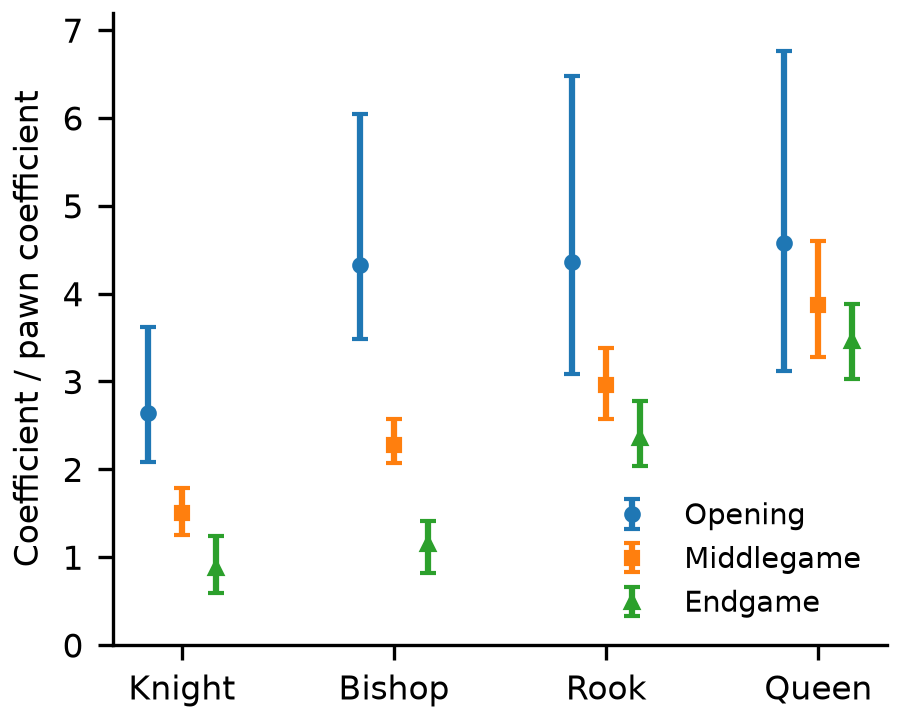
\includegraphics[width=\linewidth]{stage_values.png}
\caption{Pooled contextual IRL relative coefficients by stage. Vertical lines are pointwise 95\% intervals based on 100 game-bootstrap coefficient draws.}\label{fig:stage}
\end{figure}

\subsection{Why raw and normalized values tell different stories}
Table~\ref{tab:raw} reports the unnormalized coefficients. In particular, the pawn coefficient rises from approximately 0.636 in the opening reference population to 1.079 in the endgame population. The queen coefficient also rises, from approximately 2.911 to 3.739, even though its pawn-normalized ratio falls. Thus a decrease in a reported relative value is not evidence that the raw coefficient decreases. Normalization changes the question to value relative to the contemporaneous pawn coefficient.
\begin{table}[tbp]\centering
\small
\caption{Raw action-reward coefficients before pawn normalization. Their common numerical scale is set by temperature one and the selected regularizer.}\label{tab:raw}
\begin{tabular}{lrrr}
\toprule
Piece & Opening & Middlegame & Endgame\\\midrule
Pawn & 0.636 & 0.859 & 1.079\\
Knight & 1.681 & 1.289 & 0.943\\
Bishop & 2.751 & 1.955 & 1.241\\
Rook & 2.773 & 2.541 & 2.542\\
Queen & 2.911 & 3.322 & 3.739\\
\bottomrule\end{tabular}\end{table}
\begin{table}[tbp]\centering
\small
\caption{Endgame minus opening differences in normalized coefficients of the pooled model, using paired bootstrap draws. Intervals are exploratory, pointwise, and not multiplicity-adjusted.}\label{tab:contrast}
\begin{tabular}{lrr}
\toprule
Piece & Difference & 95\% interval\\\midrule
Knight & -1.77 & [-2.73, -0.93]\\
Bishop & -3.18 & [-5.09, -2.09]\\
Rook & -2.00 & [-4.09, -0.54]\\
Queen & -1.11 & [-3.20, 0.29]\\
\bottomrule\end{tabular}\end{table}

For knight, bishop, and rook, the paired intervals in Table~\ref{tab:contrast} exclude zero in the pooled model. The queen difference interval includes zero. These are conditional, exploratory comparisons; they do not justify a general law that each piece loses strategic value as the game progresses.


\section{Different IRL model specifications}
\subsection{Global, phase-only, openness-only, and joint models}
The global, phase-only, openness-only, and joint specifications have 8, 13, 13, and 18 parameters. All share the same immediate features, temperature convention, game-balanced objective, and validation procedure. Table~\ref{tab:family} evaluates them at the same stage reference distributions. By construction the global model cannot express stage variation. Phase-only and openness-only models attribute differences to distinct correlated covariates. Their disagreement is therefore informative about specification dependence rather than evidence that one covariate is a causal explanation.
\begin{table}[tbp]\centering
\small
\caption{Alternative specifications of the same one-step maximum-entropy IRL family, evaluated at identical stage contexts. Pawn = 1. These are not four different IRL algorithms.}\label{tab:family}
\begin{tabular}{llrrrr}
\toprule
Model & Stage & N & B & R & Q\\\midrule
Global & Opening & 1.54 & 2.22 & 2.85 & 4.00\\
Global & Middlegame & 1.54 & 2.22 & 2.85 & 4.00\\
Global & Endgame & 1.54 & 2.22 & 2.85 & 4.00\\
\addlinespace
Phase & Opening & 2.13 & 3.31 & 3.38 & 4.38\\
Phase & Middlegame & 1.53 & 2.29 & 2.89 & 3.95\\
Phase & Endgame & 0.91 & 1.22 & 2.39 & 3.51\\
\addlinespace
Openness & Opening & 2.60 & 4.26 & 4.43 & 4.57\\
Openness & Middlegame & 1.50 & 2.26 & 2.97 & 3.86\\
Openness & Endgame & 0.94 & 1.27 & 2.24 & 3.50\\
\addlinespace
Joint & Opening & 2.64 & 4.33 & 4.36 & 4.58\\
Joint & Middlegame & 1.50 & 2.28 & 2.96 & 3.87\\
Joint & Endgame & 0.87 & 1.15 & 2.36 & 3.46\\
\addlinespace
\bottomrule\end{tabular}\end{table}

These are variants of one maximum-entropy conditional-choice estimator. We do not label them as separate algorithms such as Bayesian IRL, maximum-margin IRL, or adversarial IRL. No experiments with those algorithms were run. The comparison addresses how much the relative coefficients change when context is represented differently.

\subsection{Independent estimation within each stage}
As a complementary analysis, we fit a separate eight-coefficient model to each stage's training positions. We choose ridge strength from the same three-value grid using that stage's validation positions, and perform 100 training-game cluster-bootstrap refits per stage at the selected penalty. Each stage has its own nuisance coefficients for centrality, check, and mate. Unlike the pooled summary, these estimates do not borrow coefficient constraints from other stages.
\begin{table*}[t]\centering
\small
\caption{Independently fitted stage models: each stage has its own eight coefficients and validation-selected ridge. Brackets are 95\% intervals from 100 bootstrap refits per stage.}\label{tab:independent}
\begin{tabular}{lccc}
\toprule
Piece & Opening & Middlegame & Endgame\\\midrule
Pawn & 1.00 [1.00, 1.00] & 1.00 [1.00, 1.00] & 1.00 [1.00, 1.00]\\
Knight & 1.22 [0.29, 2.22] & 1.92 [1.64, 2.42] & 0.70 [0.13, 1.22]\\
Bishop & 3.46 [2.58, 5.47] & 2.83 [2.45, 3.47] & 0.76 [0.18, 1.33]\\
Rook & 6.81 [5.21, 11.31] & 3.41 [2.96, 4.12] & 2.00 [1.53, 2.56]\\
Queen & 4.50 [1.64, 6.80] & 4.31 [3.55, 5.19] & 3.65 [3.12, 4.50]\\
\bottomrule\end{tabular}\end{table*}

The independent opening estimates in Table~\ref{tab:independent} differ substantially from the pooled opening summary. This is a change in estimator and information sharing, not an independent replication of the same quantity. An independent model approximates the conditional choices within a stage with one fixed vector, while the pooled model uses a continuous context-dependent function learned across stages. Their different normalization denominators and nuisance coefficients can further change the ratios. Cross-stage comparisons of the independent fits should therefore be treated cautiously.

\subsection{How much direct material-choice evidence is available?}
Table~\ref{tab:support} counts positions in which at least one legal action differs in the corresponding material feature. For example, an opening position with no way to change either side's rook count does not directly distinguish rook reward weights through the material component. The opening sample contains only 13 rook-informative and 10 queen-informative positions. A wide interval or large independent opening estimate should be interpreted in light of this scarcity. The counts do not imply that all informative positions are independent observations or that the expert selected a capture.
\begin{table}[tbp]\centering
\small
\caption{Number of training positions whose candidate moves differ in each material feature. These are opportunities to constrain that coefficient, not counts of expert captures.}\label{tab:support}
\begin{tabular}{lrrrrr}
\toprule
Stage & Pawn & Knight & Bishop & Rook & Queen\\\midrule
Opening & 806 & 189 & 46 & 13 & 10\\
Middlegame & 4250 & 1542 & 986 & 653 & 272\\
Endgame & 1214 & 327 & 300 & 251 & 170\\
\bottomrule\end{tabular}\end{table}


\section{Sensitivity analyses}
\subsection{Regularization strength}
Table~\ref{tab:ridge} uses the weights already fitted at all three ridge settings in the original validation grid. The reference contexts are held fixed. This separates numerical regularization sensitivity from changes in stage composition. Larger ridge penalties shrink raw coefficients, but ratios need not shrink uniformly because both numerator and pawn denominator change. We report every grid setting, including those not selected by validation, rather than selecting the most intuitive value table.
\begin{table}[tbp]\centering
\small
\caption{Ridge sensitivity of the pooled joint model at the same reference contexts. No test results were used to select these settings; all three original grid values are displayed.}\label{tab:ridge}
\begin{tabular}{rlrrrr}
\toprule
$\lambda$ & Stage & N & B & R & Q\\\midrule
0.0001 & Opening & 2.64 & 4.33 & 4.36 & 4.58\\
0.0001 & Middlegame & 1.50 & 2.28 & 2.96 & 3.87\\
0.0001 & Endgame & 0.87 & 1.15 & 2.36 & 3.46\\
\addlinespace
0.001 & Opening & 2.52 & 3.97 & 3.89 & 4.38\\
0.001 & Middlegame & 1.51 & 2.31 & 2.90 & 3.76\\
0.001 & Endgame & 0.89 & 1.25 & 2.33 & 3.39\\
\addlinespace
0.01 & Opening & 1.94 & 2.85 & 2.66 & 2.70\\
0.01 & Middlegame & 1.45 & 2.17 & 2.43 & 2.62\\
0.01 & Endgame & 1.02 & 1.58 & 2.24 & 2.55\\
\addlinespace
\bottomrule\end{tabular}\end{table}

For the original pooled models, the selected penalties lie on the lower boundary of the tested grid. The study does not establish optimality over penalties outside that grid. The displayed sensitivity is descriptive and does not supply confidence intervals for choosing between regularizers.

\subsection{Stage-boundary sensitivity}
We vary the last opening full move from 10 to 8 or 12, and the endgame material threshold from 6 to 4 or 8, changing one definition at a time. Table~\ref{tab:boundary} shows all settings. The fitted joint model is unchanged: these results measure changes in the reference population, not new IRL training runs. Consequently, similar numbers across nearby cutoffs demonstrate local stability of this summary procedure, not robustness to an entirely different model or dataset.
\begin{table}[tbp]\centering
\small
\caption{Sensitivity to the stage definition. Settings are opening last full move / endgame material-unit threshold. The model is frozen; only the reference populations change. Pawn = 1.}\label{tab:boundary}
\begin{tabular}{llrrrr}
\toprule
Definition & Stage & N & B & R & Q\\\midrule
10 / 6 & Opening & 2.64 & 4.33 & 4.36 & 4.58\\
10 / 6 & Middlegame & 1.50 & 2.28 & 2.96 & 3.87\\
10 / 6 & Endgame & 0.87 & 1.15 & 2.36 & 3.46\\
\addlinespace
8 / 6 & Opening & 2.75 & 4.53 & 4.52 & 4.64\\
8 / 6 & Middlegame & 1.55 & 2.36 & 3.01 & 3.90\\
8 / 6 & Endgame & 0.87 & 1.15 & 2.36 & 3.46\\
\addlinespace
12 / 6 & Opening & 2.54 & 4.14 & 4.22 & 4.51\\
12 / 6 & Middlegame & 1.45 & 2.19 & 2.91 & 3.84\\
12 / 6 & Endgame & 0.87 & 1.15 & 2.36 & 3.46\\
\addlinespace
10 / 4 & Opening & 2.64 & 4.33 & 4.36 & 4.58\\
10 / 4 & Middlegame & 1.39 & 2.07 & 2.84 & 3.80\\
10 / 4 & Endgame & 0.83 & 1.07 & 2.31 & 3.44\\
\addlinespace
10 / 8 & Opening & 2.64 & 4.33 & 4.36 & 4.58\\
10 / 8 & Middlegame & 1.61 & 2.47 & 3.07 & 3.94\\
10 / 8 & Endgame & 0.90 & 1.20 & 2.37 & 3.48\\
\addlinespace
\bottomrule\end{tabular}\end{table}


\section{Independent IRL by Remaining-Piece Count}
\subsection{Definition and fitting design}
To examine positions with many and few pieces directly, let $C(s)$ be the number of occupied squares minus two. Both colors and all pawns are counted, while the kings are excluded. Thus the initial position has $C=30$. Sparse positions have $C\leq10$, dense positions have $C\geq22$, and the intermediate group contains $11\leq C\leq21$. These cutoffs were specified before executing this extension, after the earlier stage analysis had been observed. They were not chosen by searching for the largest contrast.

We fit a separate eight-coefficient model in each group using the original training partition. Every group has its own material and nuisance coefficients. Its ridge penalty is selected using only its corresponding validation subset. No state is assigned to a different game split, and all three count groups jointly cover every retained state. Table~\ref{tab:countcoverage} gives their sample sizes. A game can enter more than one group, so adding the group-level game counts would overstate the number of independent games.
\begin{table*}[t]\centering
\small
\caption{Remaining-piece-count groups. Entries are positions (games). A game can contribute to several groups.}\label{tab:countcoverage}
\begin{tabular}{lrrr}
\toprule
Group & Train & Validation & Test\\\midrule
Sparse & 4,232 (147) & 1,319 (51) & 1,642 (53)\\
Intermediate & 3,354 (172) & 1,219 (60) & 1,217 (59)\\
Dense & 3,209 (179) & 1,086 (60) & 1,073 (60)\\
\bottomrule\end{tabular}\end{table*}

This analysis differs from summarizing the pooled model at a new reference context: every count-group coefficient is re-estimated from that group's demonstrations. It also differs from the original independent stage fits because the grouping variable counts pawns and gives every non-king piece equal weight. The phrase dense describes occupancy only; it does not assert that a position is strategically closed, tactically complicated, or difficult for an engine. Likewise, sparse positions are not assumed to be solved tablebase positions.

\subsection{Paired uncertainty and the primary comparison}
For uncertainty, we draw 100 bootstrap samples of the full set of 179 represented training games. Each draw supplies the same game multiplicity to every count group. Within a group, the original equal-game position weights are multiplied by those multiplicities and normalized again to sum to one. We refit at the selected penalty and compute pawn-normalized coefficients. This pairing preserves the dependence created when one game contributes both dense and sparse states. It does not create additional games, resample engine versions, or include uncertainty from hyperparameter selection.

Table~\ref{tab:countvalues} reports the resulting estimates. The sparse/dense knight ratios are 0.40 and 1.89, bishop ratios 0.96 and 3.29, rook ratios 1.98 and 3.39, and queen ratios 3.41 and 4.35. These are model-conditional descriptions of different state populations. The sparse knight interval crosses zero. A negative coefficient in a bootstrap draw is possible because material weights are not constrained to be positive; it is not a claim that removing a knight has a positive strategic value.
\begin{table*}[t]\centering
\small
\caption{Independently fitted piece-count models: pawn-normalized coefficients and pointwise 95\% intervals from 100 paired game-bootstrap draws.}\label{tab:countvalues}
\begin{tabular}{lccc}
\toprule
Piece & Sparse & Intermediate & Dense\\\midrule
Pawn & 1.00 [1.00, 1.00] & 1.00 [1.00, 1.00] & 1.00 [1.00, 1.00]\\
Knight & 0.40 [-0.33, 0.81] & 1.43 [1.18, 1.78] & 1.89 [1.52, 2.48]\\
Bishop & 0.96 [0.34, 1.39] & 1.97 [1.77, 2.48] & 3.29 [2.78, 4.17]\\
Rook & 1.98 [1.60, 2.40] & 2.73 [2.40, 3.28] & 3.39 [2.64, 4.42]\\
Queen & 3.41 [2.77, 4.38] & 3.57 [3.16, 4.28] & 4.35 [3.46, 5.61]\\
\bottomrule\end{tabular}\end{table*}

All sampled pawn coefficients exceed the prespecified numerical threshold, so normalization is retained. Table~\ref{tab:countcontrast} reports paired sparse-minus-dense differences. The knight, bishop, and rook intervals exclude zero in this exploratory comparison. The queen interval includes zero. We therefore do not describe all four types as having a statistically established decline, and none of these intervals is adjusted for the full set of analyses in the paper.
\begin{table}[tbp]\centering
\small
\caption{Paired sparse-minus-dense differences in normalized coefficients. Intervals are exploratory pointwise 95\% intervals.}\label{tab:countcontrast}
\begin{tabular}{lrr}
\toprule
Piece & Difference & Interval\\\midrule
Knight & -1.48 & [-2.15, -1.00]\\
Bishop & -2.33 & [-3.30, -1.55]\\
Rook & -1.41 & [-2.65, -0.44]\\
Queen & -0.94 & [-2.48, 0.37]\\
\bottomrule\end{tabular}\end{table}

The intermediate estimates are useful because a two-group comparison alone could obscure how the omitted middle population behaves. Here the knight, bishop, and rook point estimates fall between the sparse and dense estimates. That ordering is descriptive and should not be promoted to a monotonic law over individual piece counts. Each group still contains heterogeneous material compositions, and an independent model compresses those positions into one shared vector. A model with one coefficient for every exact count would ask a different question and require stronger support for each additional parameter.

\subsection{Raw coefficients and changing denominators}
Table~\ref{tab:countraw} retains the fitted raw coefficients. The pawn coefficient is approximately 1.137 in sparse states and 0.746 in dense states. The queen coefficient moves in the opposite direction to its normalized ratio: its raw value is approximately 3.880 in sparse states and 3.247 in dense states. Consequently, the lower sparse queen-to-pawn ratio cannot by itself be described as a smaller raw queen contribution. The same distinction applies whenever normalized tables are compared across independently fitted models.
\begin{table}[tbp]\centering
\small
\caption{Unnormalized coefficients for piece-count fits, including nuisance features.}\label{tab:countraw}
\begin{tabular}{lrrr}
\toprule
Feature & Sparse & Intermediate & Dense\\\midrule
Pawn & 1.137 & 0.992 & 0.746\\
Knight & 0.459 & 1.420 & 1.409\\
Bishop & 1.089 & 1.958 & 2.452\\
Rook & 2.254 & 2.710 & 2.533\\
Queen & 3.880 & 3.540 & 3.247\\
Center & 0.380 & 0.605 & 0.901\\
Check & 0.947 & 0.581 & -0.266\\
Mate & 6.252 & 4.569 & 0.000\\
\bottomrule\end{tabular}\end{table}

Nuisance coefficients are included to show that the material terms are fitted jointly with other explanations of the move. A check coefficient can be negative in a restricted group without implying that checking the opponent is intrinsically harmful. Conditional associations depend on which checks are available and selected, and omitted continuations can shift those associations. Similarly, a zero mate coefficient under ridge can result from the absence of differentiating mate opportunities. These terms are reported for transparency, not folded into material ratios or interpreted as independently identified chess principles.

\subsection{Overlap with stages and available evidence}
Table~\ref{tab:countoverlap} quantifies the overlap with the earlier stage partition. Of the 4,232 sparse training positions, 3,437 are endgames and 795 are middlegames. The dense group contains all 1,071 retained opening positions and 2,138 middlegame positions, with no endgames. The remaining 546 endgame positions belong to the intermediate count group. Thus the count analysis is related to, but is not identical to, the stage analysis. Its findings must not be counted as evidence from a new collection.
\begin{table}[tbp]\centering
\small
\caption{Training-state overlap between count groups and stage labels. These are position counts, not independent games.}\label{tab:countoverlap}
\begin{tabular}{lrrr}
\toprule
Group & Opening & Middle & Endgame\\\midrule
Sparse & 0 & 795 & 3437\\
Intermediate & 0 & 2808 & 546\\
Dense & 1071 & 2138 & 0\\
\bottomrule\end{tabular}\end{table}

The training groups also differ in their candidate actions and pawn structure. Their equal-game mean legal-action counts are approximately 18.37, 29.37, and 34.55 from sparse to dense. Mean file openness is approximately 0.912, 0.656, and 0.277. These simultaneous changes prevent a causal interpretation in which only piece count changes. Even if two positions have the same count, their available captures, promotions, checks, and quiet moves may be very different. The analysis compares those observed bundles of circumstances.

Table~\ref{tab:countsupport} reports states with at least one candidate difference in each material component. A state with no variation in a component provides no direct likelihood information for that coefficient through the material term. In the dense group, only 75 training positions distinguish queen-count alternatives, compared with 211 in the sparse group. Larger total sample size therefore does not automatically mean stronger information about every piece. These are opportunities to constrain a coefficient; they are not counts of selected captures or independent observations.
\begin{table}[tbp]\centering
\small
\caption{Training positions whose legal alternatives vary in each material feature.}\label{tab:countsupport}
\begin{tabular}{lrrrrr}
\toprule
Group & P & N & B & R & Q\\\midrule
Sparse & 1199 & 362 & 325 & 312 & 211\\
Intermediate & 2394 & 784 & 605 & 459 & 166\\
Dense & 2677 & 912 & 402 & 146 & 75\\
\bottomrule\end{tabular}\end{table}

\subsection{Penalty and boundary sensitivity}
The selected penalty is $10^{-4}$ for sparse and intermediate groups but $10^{-3}$ for the dense group. The dense estimate is not obtained by imposing the penalty selected for a different population. Changing regularization can alter both numerator and denominator, and the selected value need not make a ratio most similar to a conventional chess table.

We additionally refit sparse cutoffs of 8 and 12 and dense cutoffs of 20 and 24. These fits repeat within-subset validation selection and do not reuse a pooled coefficient without refitting. Table~\ref{tab:countsensitivity} reports every setting. The sparse knight ratio changes from approximately 0.40 at cutoff 8 to 0.83 at cutoff 12, showing that a single low sparse estimate is boundary-sensitive. The corresponding queen ratios are near 3.44 and 3.42. The dense alternatives also change the relative coefficients. These comparisons have no bootstrap intervals and cannot establish that every observed numerical difference is statistically meaningful.
\begin{table}[tbp]\centering
\small
\caption{Refitted boundary sensitivity. These estimates have no bootstrap intervals; all thresholds were specified before the count extension was executed.}\label{tab:countsensitivity}
\begin{tabular}{lrrrr}
\toprule
Subset & N & B & R & Q\\\midrule
$C\leq 8$ & 0.40 & 0.99 & 2.06 & 3.44\\
$C\leq 12$ & 0.83 & 1.00 & 2.35 & 3.42\\
$C\geq 20$ & 1.82 & 2.94 & 3.50 & 4.25\\
$C\geq 24$ & 1.81 & 3.37 & 3.71 & 3.96\\
\bottomrule\end{tabular}\end{table}

\subsection{Interpretation}
The new analysis supports a limited conclusion. Under this feature set and these operational groups, relative minor-piece and rook coefficients differ between sparse and dense populations, while uncertainty and denominator changes complicate the queen comparison. It does not show that the same piece in the same strategic situation loses value when unrelated pieces are removed. A design aimed at that causal question would need matched or controlled position transformations, with legality and downstream tactical effects explicitly handled. Here the descriptive group comparison is the intended result.

\section{Stockfish Strength-Setting Experiment}
\subsection{Common-position comparison}
We extend the behavioral comparison to Stockfish 18 with \texttt{UCI\_LimitStrength=true} and \texttt{UCI\_Elo} settings 1500, 2000, and 2500. The installed engine exposes a supported range of 1320--3190. The official documentation explains that the setting targets a calibrated engine strength under specified time-control conditions \cite{stockfishuci}. Our fixed 5,000-node searches do not reproduce those calibration conditions. We therefore use the numbers strictly as engine-setting labels, not as measured Elo, human skill groups, or a verified ranking of tournament performance.

Each setting is queried on exactly the same 18,351 retained positions, with one thread, a 64 MB hash, and a fresh engine game context for every query. Boards are reconstructed from FEN; full repetition histories are not restored. The original game-level split and all legal candidate features are retained; only the selected-move labels change. This design reduces the confounding that would arise if each weakened engine generated its own different self-play state distribution. It also limits generalization: the common states were visited by the original stronger engine, and may not represent positions naturally encountered by lower-strength players.

We store every returned legal move and verify its alignment with the original FEN and game identifier. Weakened move selection can be stochastic, and the exposed engine interface does not provide a seed for reproducing that component. The archived choices are therefore the exact labels for refitting. Re-querying the same positions is a new label realization, not a promised bit-for-bit recreation. The initial proposed 1320 setting was excluded when the final experimental scope was narrowed; it is not included in any reported comparison.

\subsection{Fitting and uncertainty}
For each setting, global and joint contextual models are independently trained from its selected moves. Ridge is chosen from the same three-value grid using the matching validation labels; all selected penalties are $10^{-4}$. We then refit the selected joint model for 100 training-game bootstrap samples. The identical sequence of sampled games is used across settings, preserving pairing on the common state population. These intervals condition on the archived expert-label realization and the selected penalty. They do not measure variability from repeatedly sampling the engine's weakened move selector.

Table~\ref{tab:elovalues} summarizes the joint models at a single common context: the equal-game mean of all original training states. This keeps the reference population fixed across settings. Table~\ref{tab:eloraw} retains the raw material coefficients before dividing by the pawn term. As elsewhere, ratios are shown only when the fitted pawn term and every bootstrap denominator exceed 0.001. These checks prevent numerical division by a near-zero or sign-changing denominator, but do not establish a unique underlying reward.
\begin{table*}[t]\centering
\small
\caption{Joint contextual IRL at one common all-training-state reference context. Pawn-normalized coefficients with pointwise 95\% game-bootstrap intervals. Column headings are Stockfish settings, not measured human ratings.}\label{tab:elovalues}
\begin{tabular}{lccc}
\toprule
Piece & 1500 & 2000 & 2500\\\midrule
Pawn & 1.00 [1.00, 1.00] & 1.00 [1.00, 1.00] & 1.00 [1.00, 1.00]\\
Knight & 1.49 [1.10, 2.08] & 2.02 [1.50, 2.83] & 1.53 [1.18, 2.03]\\
Bishop & 3.04 [2.32, 4.13] & 3.21 [2.52, 4.21] & 2.53 [2.04, 3.12]\\
Rook & 4.14 [3.15, 5.78] & 4.49 [3.61, 6.04] & 3.66 [3.06, 4.52]\\
Queen & 5.21 [3.94, 7.26] & 5.65 [4.34, 7.70] & 4.72 [4.03, 5.99]\\
\bottomrule\end{tabular}\end{table*}
\begin{table}[tbp]\centering
\small
\caption{Raw joint material coefficients at the common overall reference context.}\label{tab:eloraw}
\begin{tabular}{lrrr}
\toprule
Piece & 1500 & 2000 & 2500\\\midrule
Pawn & 0.439 & 0.440 & 0.585\\
Knight & 0.656 & 0.891 & 0.897\\
Bishop & 1.336 & 1.412 & 1.482\\
Rook & 1.820 & 1.978 & 2.142\\
Queen & 2.291 & 2.488 & 2.761\\
\bottomrule\end{tabular}\end{table}

The normalized point estimates are setting 1500: knight 1.49, bishop 3.04, rook 4.14, queen 5.21; setting 2000: knight 2.02, bishop 3.21, rook 4.49, queen 5.65; setting 2500: knight 1.53, bishop 2.53, rook 3.66, queen 4.72. These results answer how the restricted choice model responds to the different saved demonstrations on the same boards. They should not be interpreted as a table of what human players at those ratings believe a piece is worth. A weakened engine changes its move-selection procedure; that mechanism is not a model of human mistakes, learning, or judgment.

None of the four non-pawn paired intervals excludes zero. Table~\ref{tab:elocontrast} reports every contrast; these intervals are not adjusted for multiple comparisons.
\begin{table}[tbp]\centering
\small
\caption{Paired setting-2500 minus setting-1500 differences at the common overall reference context; exploratory pointwise 95\% intervals.}\label{tab:elocontrast}
\begin{tabular}{lrr}
\toprule
Piece & Difference & Interval\\\midrule
Knight & 0.04 & [-0.52, 0.49]\\
Bishop & -0.51 & [-1.76, 0.17]\\
Rook & -0.48 & [-2.07, 0.45]\\
Queen & -0.50 & [-2.24, 0.58]\\
\bottomrule\end{tabular}\end{table}

\subsection{Stage summaries and behavior diagnostics}
Table~\ref{tab:elostages} evaluates each fitted joint model at the original opening, middlegame, and endgame reference contexts. All nine cells use fixed contexts, and each setting has only one fitted joint coefficient vector. Therefore this table is a contextual summary, unlike the independently fitted count-group models. Its purpose is to reveal how the same fitted setting contrast is expressed at different state populations, not to multiply the number of independent experiments.

The opening ratios at settings 1500 and 2000 are withheld because their bootstrap pawn denominators fail the positivity threshold. These missing normalized entries reflect instability of the relative scale, not missing engine queries or an absence of pieces. The raw coefficients and all bootstrap draws remain available in the public results.
\begin{table}[tbp]\centering
\small
\caption{Strength-setting comparison at the same original stage reference contexts. These are pooled-model summaries, not independent cell fits. Dashes indicate failed pawn-denominator stability checks.}\label{tab:elostages}
\begin{tabular}{rlrrrr}
\toprule
Setting & Stage & N & B & R & Q\\\midrule
1500 & Opening & -- & -- & -- & --\\
1500 & Middlegame & 1.86 & 3.52 & 4.63 & 5.78\\
1500 & Endgame & 0.53 & 1.61 & 2.48 & 3.34\\
2000 & Opening & -- & -- & -- & --\\
2000 & Middlegame & 2.54 & 3.82 & 5.04 & 6.28\\
2000 & Endgame & 0.70 & 1.49 & 2.80 & 3.82\\
2500 & Opening & 2.86 & 5.12 & 5.36 & 6.31\\
2500 & Middlegame & 1.69 & 2.77 & 3.67 & 4.74\\
2500 & Endgame & 0.89 & 1.43 & 3.22 & 4.28\\
\bottomrule\end{tabular}\end{table}

Table~\ref{tab:eloagree} reports agreement between the selected moves themselves, before fitting IRL. Because the states and legal alternatives are shared, disagreement directly documents a change in the available behavioral labels. Agreement includes both the systematic effect of the setting and the randomness of weakened selection in the saved realization. It cannot separate those two sources, and a low agreement rate does not quantify a difference in playing strength.
\begin{table}[tbp]\centering
\small
\caption{Agreement between saved expert moves on the same test positions, weighted equally by game.}\label{tab:eloagree}
\begin{tabular}{rrr}
\toprule
Setting A & Setting B & Agreement\\\midrule
1500 & 2000 & 22.30\%\\
1500 & 2500 & 22.87\%\\
2000 & 2500 & 30.50\%\\
\bottomrule\end{tabular}\end{table}

\subsection{What this extension adds}
The experiment changes the demonstrated actions while preserving the observed board population, complementing the count analysis that changes the fitted state subset. Together, the two extensions distinguish two sources of variation in an estimated coefficient: which decisions the demonstrator makes on a given set of boards, and which boards the estimator is asked to summarize. Neither source is an intrinsic property of the piece alone. In particular, there is no requirement that increasing the nominal setting makes every ratio converge monotonically to a conventional hand-assigned value.

The comparison remains limited by one engine family, one search budget, and one draw of weakened labels. Independent repeats would be needed to estimate engine-selector variability. A human-rating study would require human games with a specified platform, rating system, and time control. These additional designs are not substituted by the three numerical labels used here. The contribution of the present extension is a controlled common-position behavioral comparison with reproducible saved labels and model-conditional uncertainty.

\section{Limitations and conclusion}
The paper estimates model-conditional, stage-specific relative piece values within a horizon-one IRL family. Immediate feature differences cannot represent a future recapture, a mating combination several plies away, or the long-term benefit of retaining a piece. Quiet non-promoting moves usually have zero material difference. Missing continuations and omitted positional features can be absorbed into coefficients. These limitations explain why the tables must not be treated as universally valid strategic prices, although they do not quantify which omission causes each observed discrepancy.

The results come from one engine version, one node budget, random early exploration, one main game collection, and one train/validation/test split. Bootstrap intervals measure conditional sampling variation rather than generalization across engines or stronger search. Stage boundaries are operational, and phases differ in both material and pawn structure. The pooled and independent estimators have different sharing assumptions. All follow-up analyses were motivated after observing the original run and should be read as exploratory. There is no claim of a new IRL algorithm, a new discovery that piece values are contextual, or improved match strength.

The principal output is a transparent stage-specific value table together with comparisons that expose its dependence on estimation choices. Reporting pooled and independent fits, raw and normalized coefficients, and sensitivity to penalties and boundaries is more informative than presenting one numerical table as definitive. The data support further investigation with reply-aware features and independent collections, while the current results form a reproducible restricted baseline.

\appendix
\section{Reproducibility and numerical checks}
The original analytic-gradient check had maximum absolute error $3.75\times10^{-11}$, and a synthetic conditional-choice recovery test had coefficient RMSE 0.0386. Perspective, promotion, legal candidate enumeration, board restoration, and game weighting were tested. Collected histories were replayed to verify stored states and moves. The extension additionally verifies that stage-subset target rows equal the corresponding original chosen-action feature rows and that subset game weights sum to one.

Original bootstrap coefficients are used only for pooled stage summaries. Independent-stage intervals come from 300 additional refits, 100 per stage, with stage-specific penalties fixed after validation. Stage subsetting does not move any game across the original train/validation/test partition. Neither context cutoffs nor the displayed sensitivity settings are selected using test performance. Package versions, full configurations, code hashes, and engine hashes accompany the numerical results.

\section{Likelihood Geometry and Reproducible Inference}
Let $z_{ia}$ denote the full design vector for candidate $a$ in state $i$, including context interactions where applicable, and let $\alpha_i$ be its equal-game observation weight. With $\mu_i=\sum_a\pi_\theta(a\mid s_i)z_{ia}$, the objective gradient is
\begin{equation}
\nabla\mathcal L(\theta)=\sum_i\alpha_i(\mu_i-z_{ia_i})+\lambda\theta.
\end{equation}
The Hessian is a sum of within-state feature covariances plus the ridge contribution:
\begin{equation}
\nabla^2\mathcal L(\theta)=\sum_i\alpha_i\operatorname{Cov}_{\pi_\theta}(z_{ia})+\lambda I.
\end{equation}
This gives a direct interpretation of the support diagnostics. If a feature has the same value for every candidate in a state, its centered value is zero and that state contributes no direct covariance information in that direction. Positive ridge gives a unique penalized optimum for a fixed design, but the resulting numerical value can still be primarily penalty-driven when the likelihood is weakly informative. A large number of states is not a substitute for variation among their legal alternatives.

The pre-move feature subtraction cancels from the softmax normalizer because context is fixed before the action. Consequently, scoring post-move features or their differences gives the same choice probabilities under the same coefficients. This equivalence would not justify changing the perspective after the move: own-minus-opponent features must remain defined from the original mover's perspective. Captures and promotions are checked explicitly in the supplied numerical tests.

The public archive preserves both the game histories and the retained feature caches. The histories support replay and checking of state/action alignment; caches permit refitting without re-querying the engine. Saved bootstrap arrays reproduce reported intervals without new random draws. Protocol files identify which analyses preceded the original run and which were added afterward. The remaining-piece extension and strength-setting extension each have a dedicated verification program that recomputes saved metrics and intervals and checks the hashes of their inputs.
\FloatBarrier
\begin{small}
\authorcontributions{J.K.: Conceptualization, Methodology, Software, Validation, Formal analysis, Investigation, Data curation, Visualization, Writing---original draft, and Writing---review and editing.}
\competinginterests{The author declares that no competing interests exist.}
\aideclaration{During preparation of this work, OpenAI Codex (OpenAI; a GPT-6-based assistant) assisted with research design, software implementation, numerical analysis, manuscript drafting, translation, and formatting. Its use extended beyond language editing. Numerical results were generated by the accompanying programs. J.K. is responsible for verifying and editing the content and for the integrity of the reported research. The exact application build and extension identifiers were not recorded.}
\dataavailability{The code, 300 self-play game histories, retained-position splits, fitted coefficients, bootstrap draws, and extension results are available at \url{https://github.com/rlawjdqls1212/piece-values-irl}. The repository documents software versions, engine settings, reproduction commands, and data checksums. The original engine executable is obtained separately from the official Stockfish release.}
\funding{This research received no external funding.}
\end{small}
\bibliography{references}
\medskip
\noindent\cornersize{.2}\setlength{\fboxsep}{6pt}
\ovalbox{\begin{minipage}{\dimexpr\columnwidth-2\fboxsep-2\fboxrule-2pt\relax}
\small
\textbf{Citation:} J. Kim. \emph{Stage-Specific Relative Chess Piece Values Estimated with One-Step Maximum-Entropy IRL}. Journal of Computer Science \& Technology. Publication metadata to be assigned by the journal.\\[3pt]
\textbf{DOI:} To be assigned.\\
\textbf{Received / Accepted:} To be assigned.\\
\textbf{Copyright:} Journal publication license: CC-BY-NC-SA. This manuscript has not been accepted or published.
\end{minipage}}
\end{document}
